\section{Tasks and time planning}
\label{sec:tasks_and_time_planning}
This project intends to implement various features aimed to improve the object management stage of the COMPSs programming model. These features may depend on some previous features or they may be totally independent and disjoint. This project also requires some additional tasks, as writing this document. All tasks, with their dependencies, can be found in figure \ref{fig:thesis_task_graph}.

\begin{figure}[ht!]
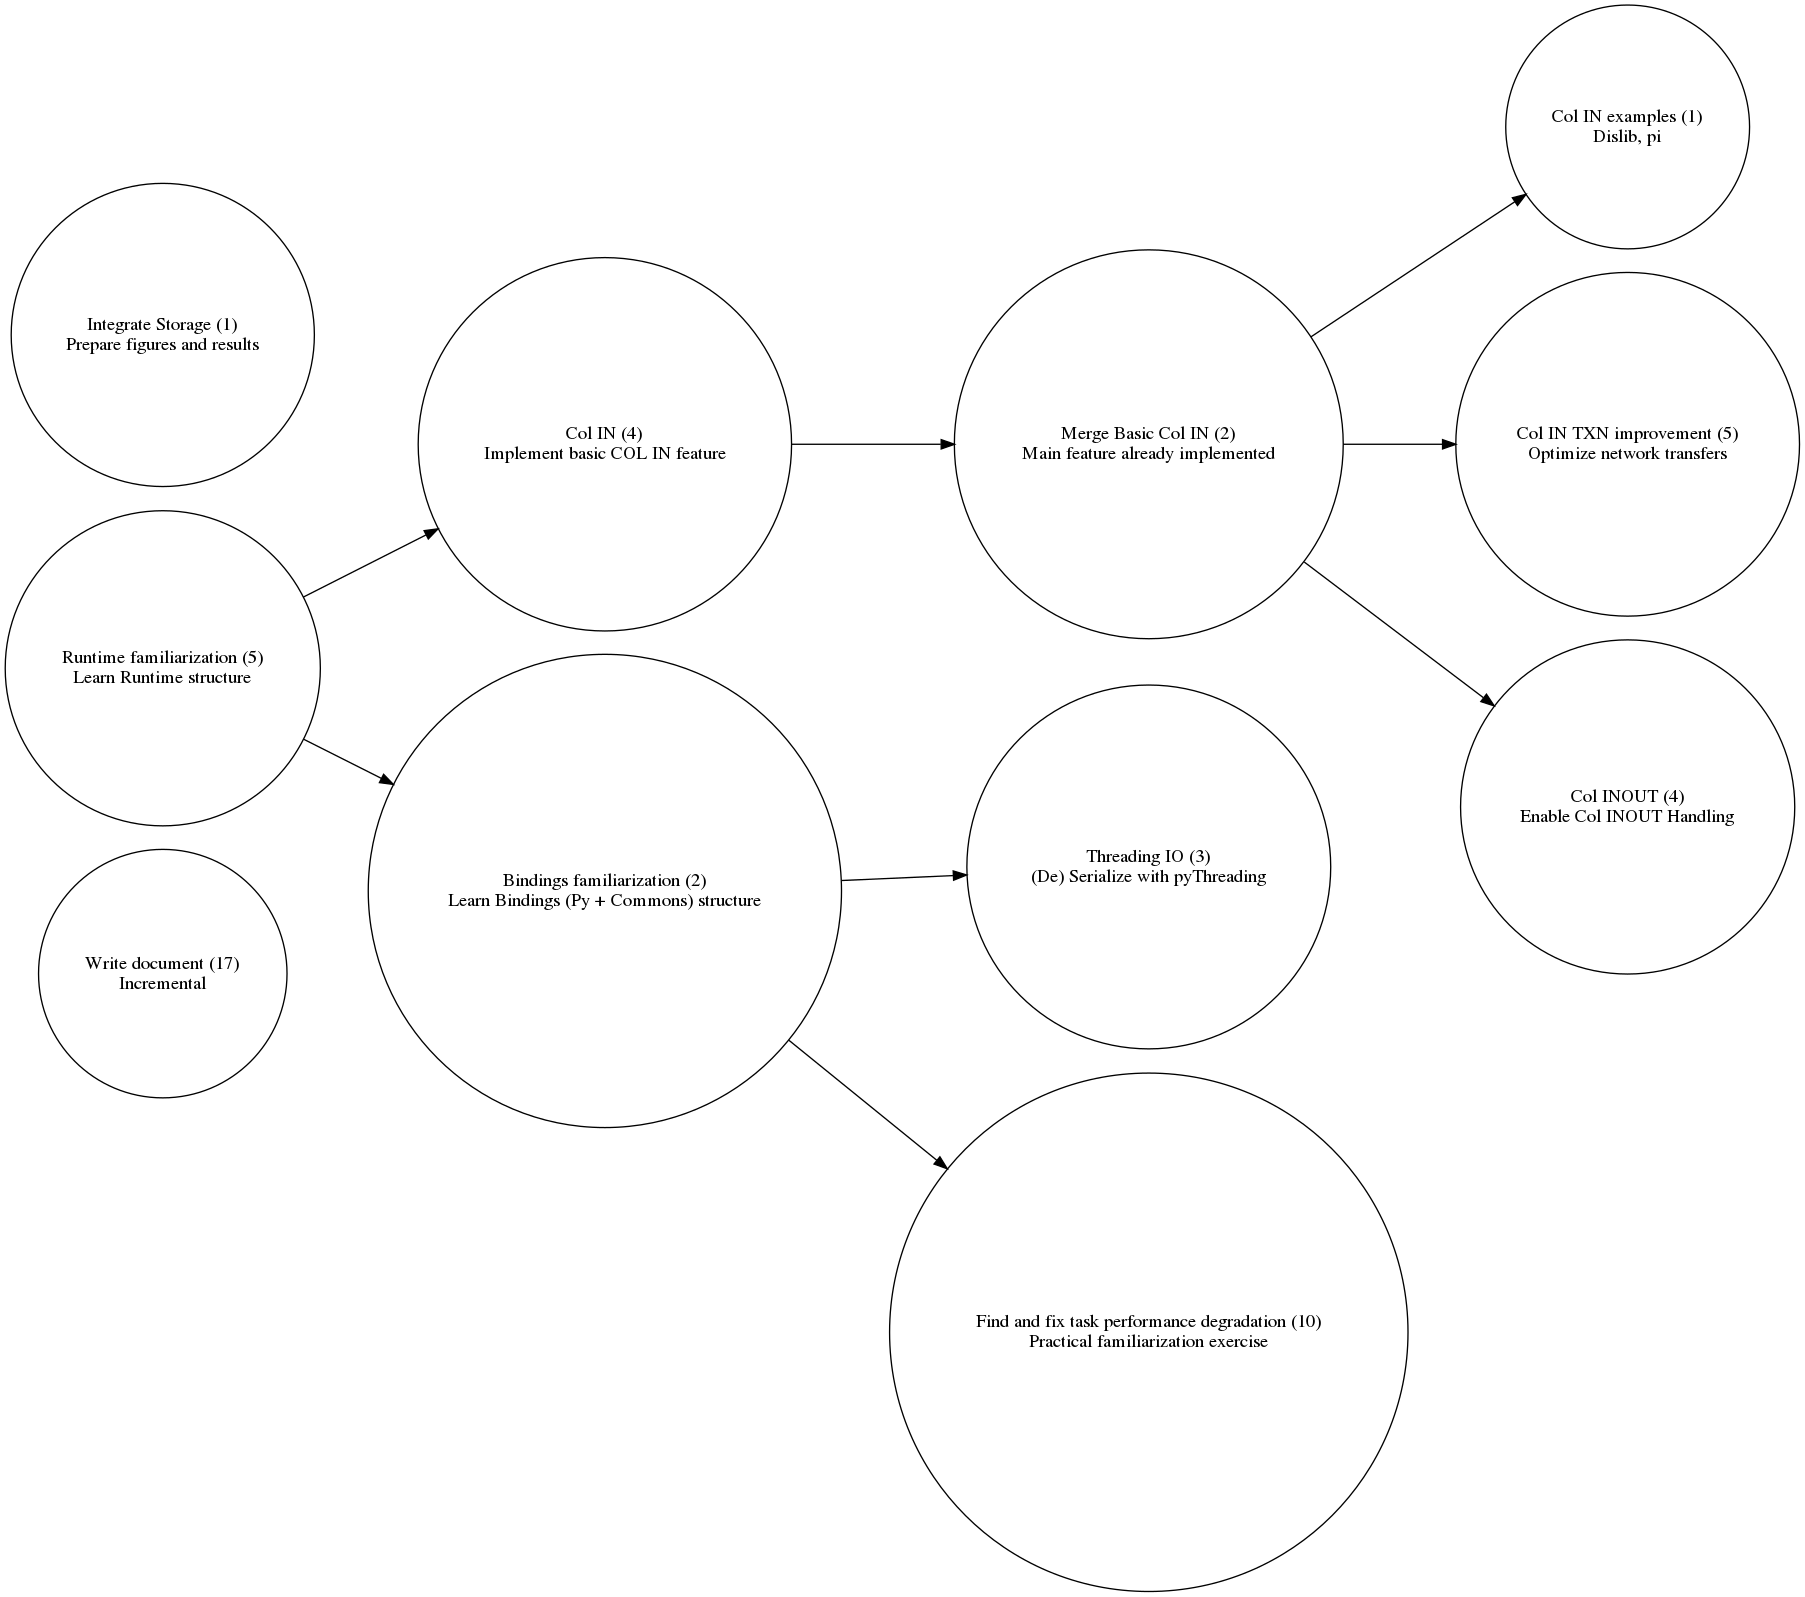
\includegraphics[scale = 0.20]{figures/thesis_task_graph.png}
\label{fig:thesis_task_graph}
\caption{A dependency graph representation of the different tasks and the dependencies between them. The numbers between parentheses denote the estimated number of needed weeks to do some task}
\end{figure}

A more precise explanation of these tasks (and shortcuts to the corresponding sections) can be found below. It is recommended to read the following sections in order to fully understand all the terms and explanations that will appear in this document.

\begin{itemize}
\item \textbf{Runtime familiarization} Some features require a deep knowledge of the COMPSs Runtime. COMPSs is written in Java, so this task will mainly consist of learning the class hierarchy and modules of the Runtime, how to build and deploy it, and how to fix and add features to it. This task is explained and developed mainly in section \ref{subsec:runtime_structure}
\item \textbf{Bindings familiarization} COMPSs has two bindings that allow the user to write applications for both C/C++ and Python. We will mainly focus on the Python (PyCOMPSs) part. This task will consist of learning the different Python modules, how user code is decorated from there, and how this binding communicates with the COMPSs Runtime via C++ Python extensions \footnote{https://docs.python.org/3/extending/building.html} and the JNI library \footnote{https://es.wikipedia.org/wiki/Java\_Native\_Interface}. The development of this task can be found in section \ref{subsec:pycompss_structure}.

\item \textbf{Col IN} This feature will allow the user to deal with multiple COMPSs parameters at once if he puts them in some container. This task and all the others that have something to do with it is developed and explained in section \ref{sec:col}.

\item \textbf{Combine Storage with PyCOMPSs} One of our approaches towards the improvement of object management is to partially delegate it to some \textit{dedicated} storage backend. This includes the development of some PyCOMPSs API that allows the user to use this backend and to integrate it to the \textit{intelligence} of the COMPSs Runtime. All the work related with this task can be found in section \ref{sec:storage}.

\item \textbf{Threading IO in PyCOMPSs} Most Python implementations have a Global Interpreter Lock (GIL) that prevent parallelism with Python threads. This does not mean that some speedup can be obtained if IO operations are done with Python threads, and that Python programs are necessary sequential or, at best, concurrent (for example, the Numpy library has many linear algebra operations implemented with OpenMP). This task explores if it is worthy to parallelize IO operations with Python threads and it can be found in section \ref{sec:threading_io}.

\end{itemize}

